\section{ロジスティック回帰とパーセプトロン}
本節では非線形回帰の一種であるロジスティック回帰 (logistic regression) および 1層パーセプトロン (perceptron) を取り扱う.
分類問題
, perceptron
\url{https://www.cs.utexas.edu/~gdurrett/courses/fa2022/perc-lr-connections.pdf}
\url{https://en.wikipedia.org/wiki/Perceptron}
\url{https://arxiv.org/abs/2012.03642}
perceptronは0/1 or -1/1のどちらか
UNDERSTANDING STRAIGHT-THROUGH ESTIMATOR IN TRAINING ACTIVATION QUANTIZED NEURAL NETS
Yoshua Bengio, Nicholas L´eonard, and Aaron Courville. Estimating or propagating gradients through stochastic neurons for conditional computation. arXiv preprint arXiv:1308.3432, 2013.
Hinton (2012) in his lecture 15b
G. Hinton. Neural networks for machine learning, 2012.
\url{https://www.cs.toronto.edu/~hinton/coursera_lectures.html}
delta rule
Here σ denotes the (point-wise) activation function, $W \in R^{m\times n}$
is the weight-matrix and $b \in R^n$
is
the bias-vector. The vector $x \in R^m$ and the vector $y \in R^n$ denote the input, respectively the output
\begin{equation}
y=\sigma(W^\top x + b)
\end{equation}
\begin{align}
& \text { Initialize } W^0, b^0 \text {; } \\
& \text { for } k=1,2, \ldots \text { do } \\
& \qquad \begin{array}{|l}
\text { for } i=1, \ldots, s \text { do } \\
e_i=y_i-\sigma\left(\left(W^k\right)^{\top} x_i+b^k\right) \\
W^{k+1}=W^k+e_i x_i^{\top} \\
b^{k+1}=b^k+e_i
\end{array} \\
& \text { end }
\end{align}
\begin{lstlisting}[language=julia]
using Random, PyPlot, ProgressMeter
rc("axes.spines", top=false, right=false)
\end{lstlisting}
\begin{lstlisting}[language=julia]
N = 400 # num of inputs
dims = 2  # dims of inputs 
Random.seed!(1234);
\end{lstlisting}
\begin{lstlisting}[language=julia]
X = [randn(Int(N/2), dims);  3.0 .+ randn(Int(N/2), dims)];
y = [zeros(Int(N/2)); ones(Int(N/2))];
\end{lstlisting}
\begin{lstlisting}[language=julia]
fig, ax = subplots(figsize=(3, 3))
for i in [0, 1]
    ax.scatter(X[y.==i, 1], X[y.==i, 2])
end
ax.set_xlabel(L"$x_1$"); ax.set_ylabel(L"$x_2$"); 
tight_layout()
\end{lstlisting}
\begin{figure}[ht]
	\centering
	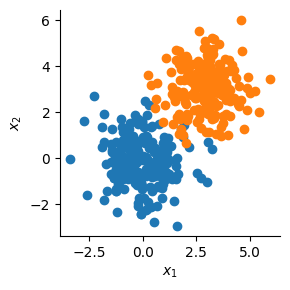
\includegraphics[scale=0.8, max width=\linewidth]{./fig/local-learning-rule/logistic-regression-perceptron/cell006.png}
	\caption{cell006.png}
	\label{cell006.png}
\end{figure}
\begin{lstlisting}[language=julia]
m, n = 2, 1
\end{lstlisting}
\begin{lstlisting}[language=julia]
step(x) = 1.0(x > 0)
\end{lstlisting}
\begin{lstlisting}[language=julia]
x = -1:0.01:1
figure(figsize=(3, 2))
plot(x, step.(x))
tight_layout()
\end{lstlisting}
\begin{figure}[ht]
	\centering
	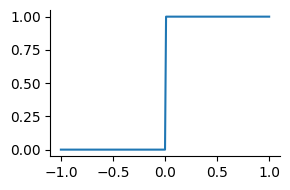
\includegraphics[scale=0.8, max width=\linewidth]{./fig/local-learning-rule/logistic-regression-perceptron/cell009.png}
	\caption{cell009.png}
	\label{cell009.png}
\end{figure}
\begin{lstlisting}[language=julia]
num_in, num_out
n, num_in = size(X)
\end{lstlisting}
\begin{lstlisting}[language=julia]
size(y)[1]
\end{lstlisting}
\begin{lstlisting}[language=julia]

\end{lstlisting}
\begin{lstlisting}[language=julia]
function perceptron(X, y; init_w=nothing, f=step, lr=0.1, num_iters=100)
    num_samples, n = size(X)
    m = 1
    if init_w == nothing
        W = randn(n, m)
        b = randn()
    end
    loss = zeros(num_iters);
    lr /= num_samples
    for t in 1:num_iters
        ŷ = f.(X * W .+ b)
        e = y - ŷ
        loss[t] = sum(e.^2) 
        W[:, :] += lr * e' * X
        b += lr * sum(e)
    end
    return W, b
end
\end{lstlisting}
\begin{lstlisting}[language=julia]
num_samples, n = size(X)
m = 1
W = randn(n, m)
b = randn()
lr = 0.1
f = step
lr /= num_samples
\end{lstlisting}
\begin{lstlisting}[language=julia]
size(X * W)
\end{lstlisting}
\begin{lstlisting}[language=julia]
b
\end{lstlisting}
\begin{lstlisting}[language=julia]
e = y - ŷ
loss[t] = sum(e.^2) 
#W[:, :] += lr * e' * X
#b[:] .+= lr * sum(e)
\end{lstlisting}
\begin{lstlisting}[language=julia]
W, b = perceptron(X, y)
\end{lstlisting}
\begin{lstlisting}[language=julia]
figure(figsize=(3,2))
plot(loss)
xlabel("Iteration"); ylabel("Loss")
tight_layout()
\end{lstlisting}
\begin{figure}[ht]
	\centering
	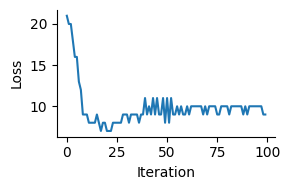
\includegraphics[scale=0.8, max width=\linewidth]{./fig/local-learning-rule/logistic-regression-perceptron/cell019.png}
	\caption{cell019.png}
	\label{cell019.png}
\end{figure}
\begin{lstlisting}[language=julia]
ŷ = step.(W * X' .+ b)'; # prediction
\end{lstlisting}
\begin{lstlisting}[language=julia]
p1 = X[ŷ[:, 1] .== 0, :]
p2 = X[ŷ[:, 1] .== 1, :];
\end{lstlisting}
ax + by + c = 0  
y = -a/b x - c/b
\begin{lstlisting}[language=julia]
xx = -3:0.01:6
yy = -W[1]/W[2]*xx .- b / W[2];
\end{lstlisting}
\begin{lstlisting}[language=julia]
figure(figsize=(4, 4))
scatter(p1[:, 1], p1[:, 2])
scatter(p2[:, 1], p2[:, 2])
plot(xx, yy, color="k")
xlabel(L"$x_1$"); ylabel(L"$x_2$"); 
tight_layout()
\end{lstlisting}
\begin{figure}[ht]
	\centering
	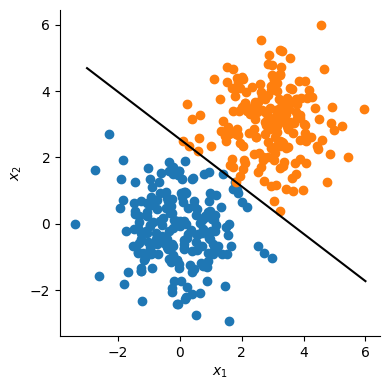
\includegraphics[scale=0.8, max width=\linewidth]{./fig/local-learning-rule/logistic-regression-perceptron/cell024.png}
	\caption{cell024.png}
	\label{cell024.png}
\end{figure}
